\Chapter{Simulations}  
%%%%%%%%%%%%%%%%%%%%%%%%%%%%%%%%%%%%%%%%%%%%%%%%%%%%%%%%%%%%%%%%%%%%%%%%%%%%%%%%
%%%%%%%%%%%%%%%%%%%%%%%%%%%%%%%%%%%%%%%%%%%%%%%%%%%%%%%%%%%%%%%%%%%%%%%%%%%%%%%%
\Section{Introduction}\label{sec:code}
%%%%%%%%%%%%%%%%%%%%%%%%%%%%%%%%%%%%%%%%%%%%%%%%%%%%%%%%%%%%%%%%%%%%%%%%%%%%%%%%
%%%%%%%%%%%%%%%%%%%%%%%%%%%%%%%%%%%%%%%%%%%%%%%%%%%%%%%%%%%%%%%%%%%%%%%%%%%%%%%%

\lsnote{{\it I updated this comment} You still need a bit more here in the summary paragraphs.  (1) Why are simulations needed?  -> for (1), you should also include that simulation determines beamline design parameters (streamlining hardware configuration) and parameter settings (saving time). Mention that AWA machine is often reconfigured, so especially important.  In SC discussion, when you say `high charge' give some numbers.  (2) What simulation work was done?  -> include a summary description of what was modeled (3) What were the results?   This suff all has to be before the first sub-section.}

With the rapid improvement in computing resources and codes in recent years,  
accelerator facilities can now strive to rely on accurate beam dynamics simulations. 
These simulations \lsnote{model \sout{include}} single particle effects 
(e.g. particle tracking in a magnetic field) as well as collective effects such as space charge (SC),  
and coherent synchrotron radiation (CSR).

The beam dynamics reported in this thesis, were simulated with 
the open source, particle-in-cell (PIC) code OPAL \cite{opal}. 
PIC codes simulate the electromagnetic forces that particles see in an accelerator. 
This is done by mapping the input particles onto a grid. 
Then in each time (or z) step, the forces due to space charge, accelerating gradients, 
and magnets are calculated and applied to the grid.
OPAL comes in two flavors, OPAL-CYC and OPAL-T. The first is used to model 
cyclotrons, and the latter, which is used for this work, is suited for photoinjectors. 
OPAL-T was chosen in part because it models the 3D space charge necessary to accurately simulate the high charge bunches at the AWA. 
It was chosen for several reasons:
\begin{itemize}
	\item \lsnote{Ability \sout{Able}} to calculate transverse space charge and wakefield forces 
	\item Option to run the code in parallel
	\item Data recorded in global and local reference frames 
	\item Free and open source (freely available to the public)
\end{itemize} 

The first item is crucial to standard operations at the AWA. Especially in the 
case of TBA, \lsnote{a} high charge is needed \lsnote{in the \sout{on}} drive beam line, therefore transverse 
space charge must be calculated in the simulations to give realistic results. \lsnote{{\it you need a sentence here giving the range of charge and typical emittance, or alternatively include in Table 1.1 and have (see Table 1.1 for beam parameters) at end of sentence. }}
The \lsnote{ability to run the code in parallel \sout{second item}} dramatically reduced the amount of simulation time needed. 
For example, simulating the gun and linac, about \SI{15}{m} of elements,
with 100,000 particles on one core would take about 30 minutes. 
When the number of cores is increased to 16, the same run takes less than 
5 minutes. This reduction in time by ~80\%, combined with the capability to run 
many cases at once on the cluster allows for more efficient use of time.
Typical running conditions were on 16 cores, for random samples up to 128 cores, 
and up to 5,200 cores for large optimization runs.\\
\lsnote{What was modeled and why goes here}\\
\lsnote{What was achieved goes here}\\  
\lsnote{summarize what follows}


%%%%%%%%%%%%%%%%%%%%%%%%%%%%%%%%%%%%%%%%%%%%%%%%%%%%%%%%%%%%%%%%%%%%%%%%%%%%%%%%
%%%%%%%%%%%%%%%%%%%%%%%%%%%%%%%%%%%%%%%%%%%%%%%%%%%%%%%%%%%%%%%%%%%%%%%%%%%%%%%%
\Section{Benchmarking}\label{sec:bench}

Initially OPAL-t was benchmarked against commonly used particle tracking codes ASTRA and GPT.  
This ensured correct use of the code, and reliability of \mbox{OPAL-t}.  
Two collective effects of particular interest to the AWA were included in the investigation: 
space charge (SC) and coherent synchrotron radiation (CSR).
The beam dynamics of a \SI{1}{nC} drive beam in the photoinjector were used as 
the model for comparison in the space charge study. 
A $20^{\circ}$ hard edge dipole magnet was used to benchmark CSR effects in GPT and OPAL-t by bending a 1nC beam 
at energies between \SI{2}{Mev} and \SI{100}{MeV}.  
The results of these benchmark studies are presented below, 
including a discussion of the similarities and differences between the codes.
 
The AWA group has used several beam codes in the past including:\\
\mbox{T-STEP/PARMELA}~\cite{parmela}, ASTRA~\cite{astra}, and GPT~\cite{gpt}.  
In order to take advantage of computing resources offered by 
Argonne National Laboratory (ANL), an investigation of 
OPAL~\cite{opal} was done; this is an open source and parallel code that comes in two flavors;  
OPAL-CYL and OPAL-t. The latter was installed on the Blues and Bebop high performance computing clusters
at the Laboratory Computing Resource Center (LCRC) provided by ANL~\cite{lcrc}.
(See Appendix~\ref{build} for instruction on how to build OPAL-t at ANL.)

\Subsection{Gun Simulations}
The SC algorithms were probed using the AWA photoinjector, 
a 1.5 cell copper standing-wave cavity at 1.3 GHz, 
with bucking, focusing, and matching solenoids. 
In the remainder of this thesis, the word gun is used 
in place of photoinjector. The simulation parameters were chosen to 
approximately generate the canonical “\lsnote{2D transverse emittance of} \SI{1}{\micro\metre} at \lsnote{bunch charge} 1 nC” case.  
The initial beam parameters were based on gun operations at PITZ \cite{pitz},
due to the similarities between the PITZ and AWA rf guns.
The PITZ parameters came close to achieving the \SI{1}{\micro\metre}
target without any optimization. A coarse 1D minimization
\nrnote{add method used here} of the 
emittance was done to determine the value of the laser radius 
used in this benchmark. The resulting minimum emittance was   
\SI{1.16}{\micro\metre}. 

The initial bunch distribution parameters as well as the 
on-axis gun gradient, and magnetic field of the solenoids used in 
the benchmark are listed in Table~\ref{tab:bench}. 
The rf gun and solenoid field maps were generated 
with the SUPERFISH/POISSON  codes~\cite{superfish}.
The gradient was chosen to match typical operations at PITZ~\cite{pitz}
and the AWA. The rf and solenoid fields seen by the beam in the gun are shown in Figure~\ref{fig:gunfields}.
\begin{table}
	\begin{center}
		\caption{Input simulation parameters for gun benchmark.}\label{tab:bench}
		\begin{tabular}{l l} 
	\toprule
	\toprule
	\textbf{Parameter} & \textbf{Value} \\ 
	\midrule
	$\sigma_x =\sigma_y$ & \SI{1}{mm} \\
	Gradient & \SI{60}{MV/m} \\
	
	Phase & Max energy (on crest) \\
	
	Laser radius & \SI{0.75}{mm} \\
	
	Rise and fall time & \SI{6}{ps} \\
	
	Initial kinetic energy & \SI{0.55}{eV} \\
	
	Matching solenoid strength & \SI{-0.389}{T} \\
	
	Buck and focusing solenoid strength & \SI{-0.12}{T} \\
	\bottomrule			
\end{tabular}
	\end{center}
\end{table}
\begin{figure}
	\begin{center}
		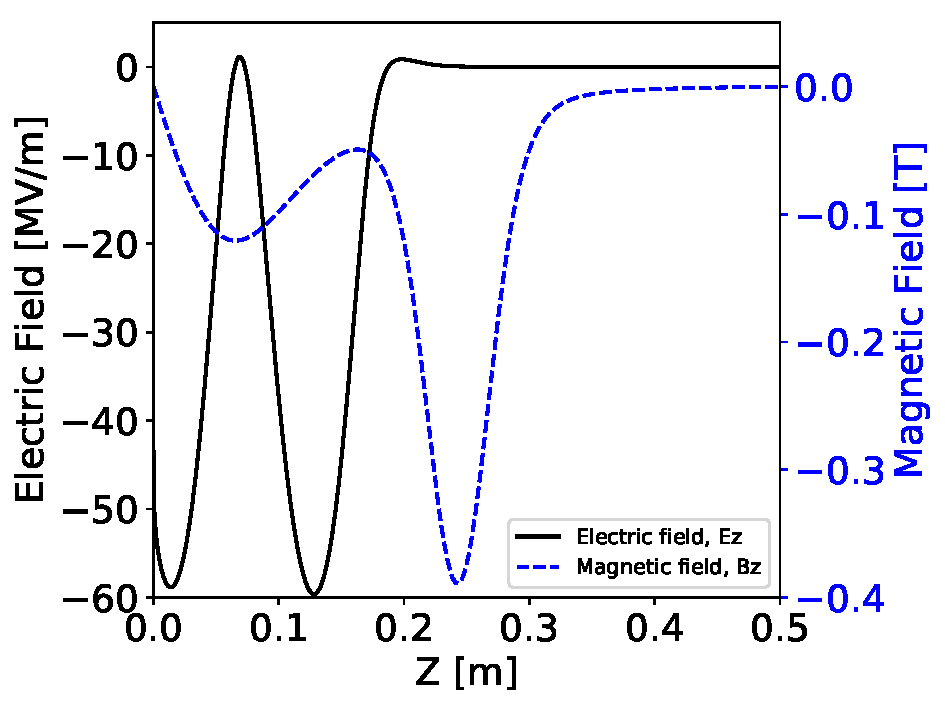
\includegraphics[width=0.75\textwidth]{images/gun_EM_fields}
		\caption{Electric and magnetic fields seen by the beam on axis in the gun. 
			The gun ends at \SI{0.3}{m}. }
		\label{fig:gunfields}
	\end{center}
\end{figure}

Note that the codes use various methods to model 
the rf and magnetic fields, SC, and image charge. 
The ASTRA simulations used the axial E field of the  
gun and solenoids, and then extended the fields to find the
transverse components using the paraxial approximation 
(e.g. $E_r=-\frac{r}{2}\frac{dE_z}{dz}$). 
The simulation used a 2D cylindrical-symmetric SC algorithm with a uniform  
particle-deposition mesh; see ASTRA user manual~\cite{astra}.
The radial and longitudinal number of cells composing the mesh 
were $N_r=32$ and $N_z=64$, with 100k particles.  
The image charge close to the cathode was accounted for until 
the bunch reached \SI{9.7}{cm} from the cathode surface. 

GPT read in the 2D electric and magnetic field files,  
and used a square 3D adaptive SC mesh with $N_x=N_y=N_z=46$
with 100k particles, see spacecharge3Dmesh option in GPT manual~\cite{gpt}.
To calculate image charge, GPT uses a Dirichlet boundary condition at the  
cathode (z=0). The calculation is turned off when the  
distance between the beam and cathode is longer than the 
mesh box. OPAL-T also read in the field maps, and used a block 
structured equidistant SC mesh, see OPAL manual for SC calculation~\cite{opal}.  
Several square mesh sizes were run in OPAL-T. The results plotted in 
Figure~\ref{fig:benchplot_gun} and~\ref{fig:benchplot_5m} correspond to a mesh of $N_x=N_y=N_z=46$, with 1 million particles. 
The image charge calculation uses a 
shifted integrated Green function \cite{imagecharge}.  
\begin{figure}
	\begin{center}
		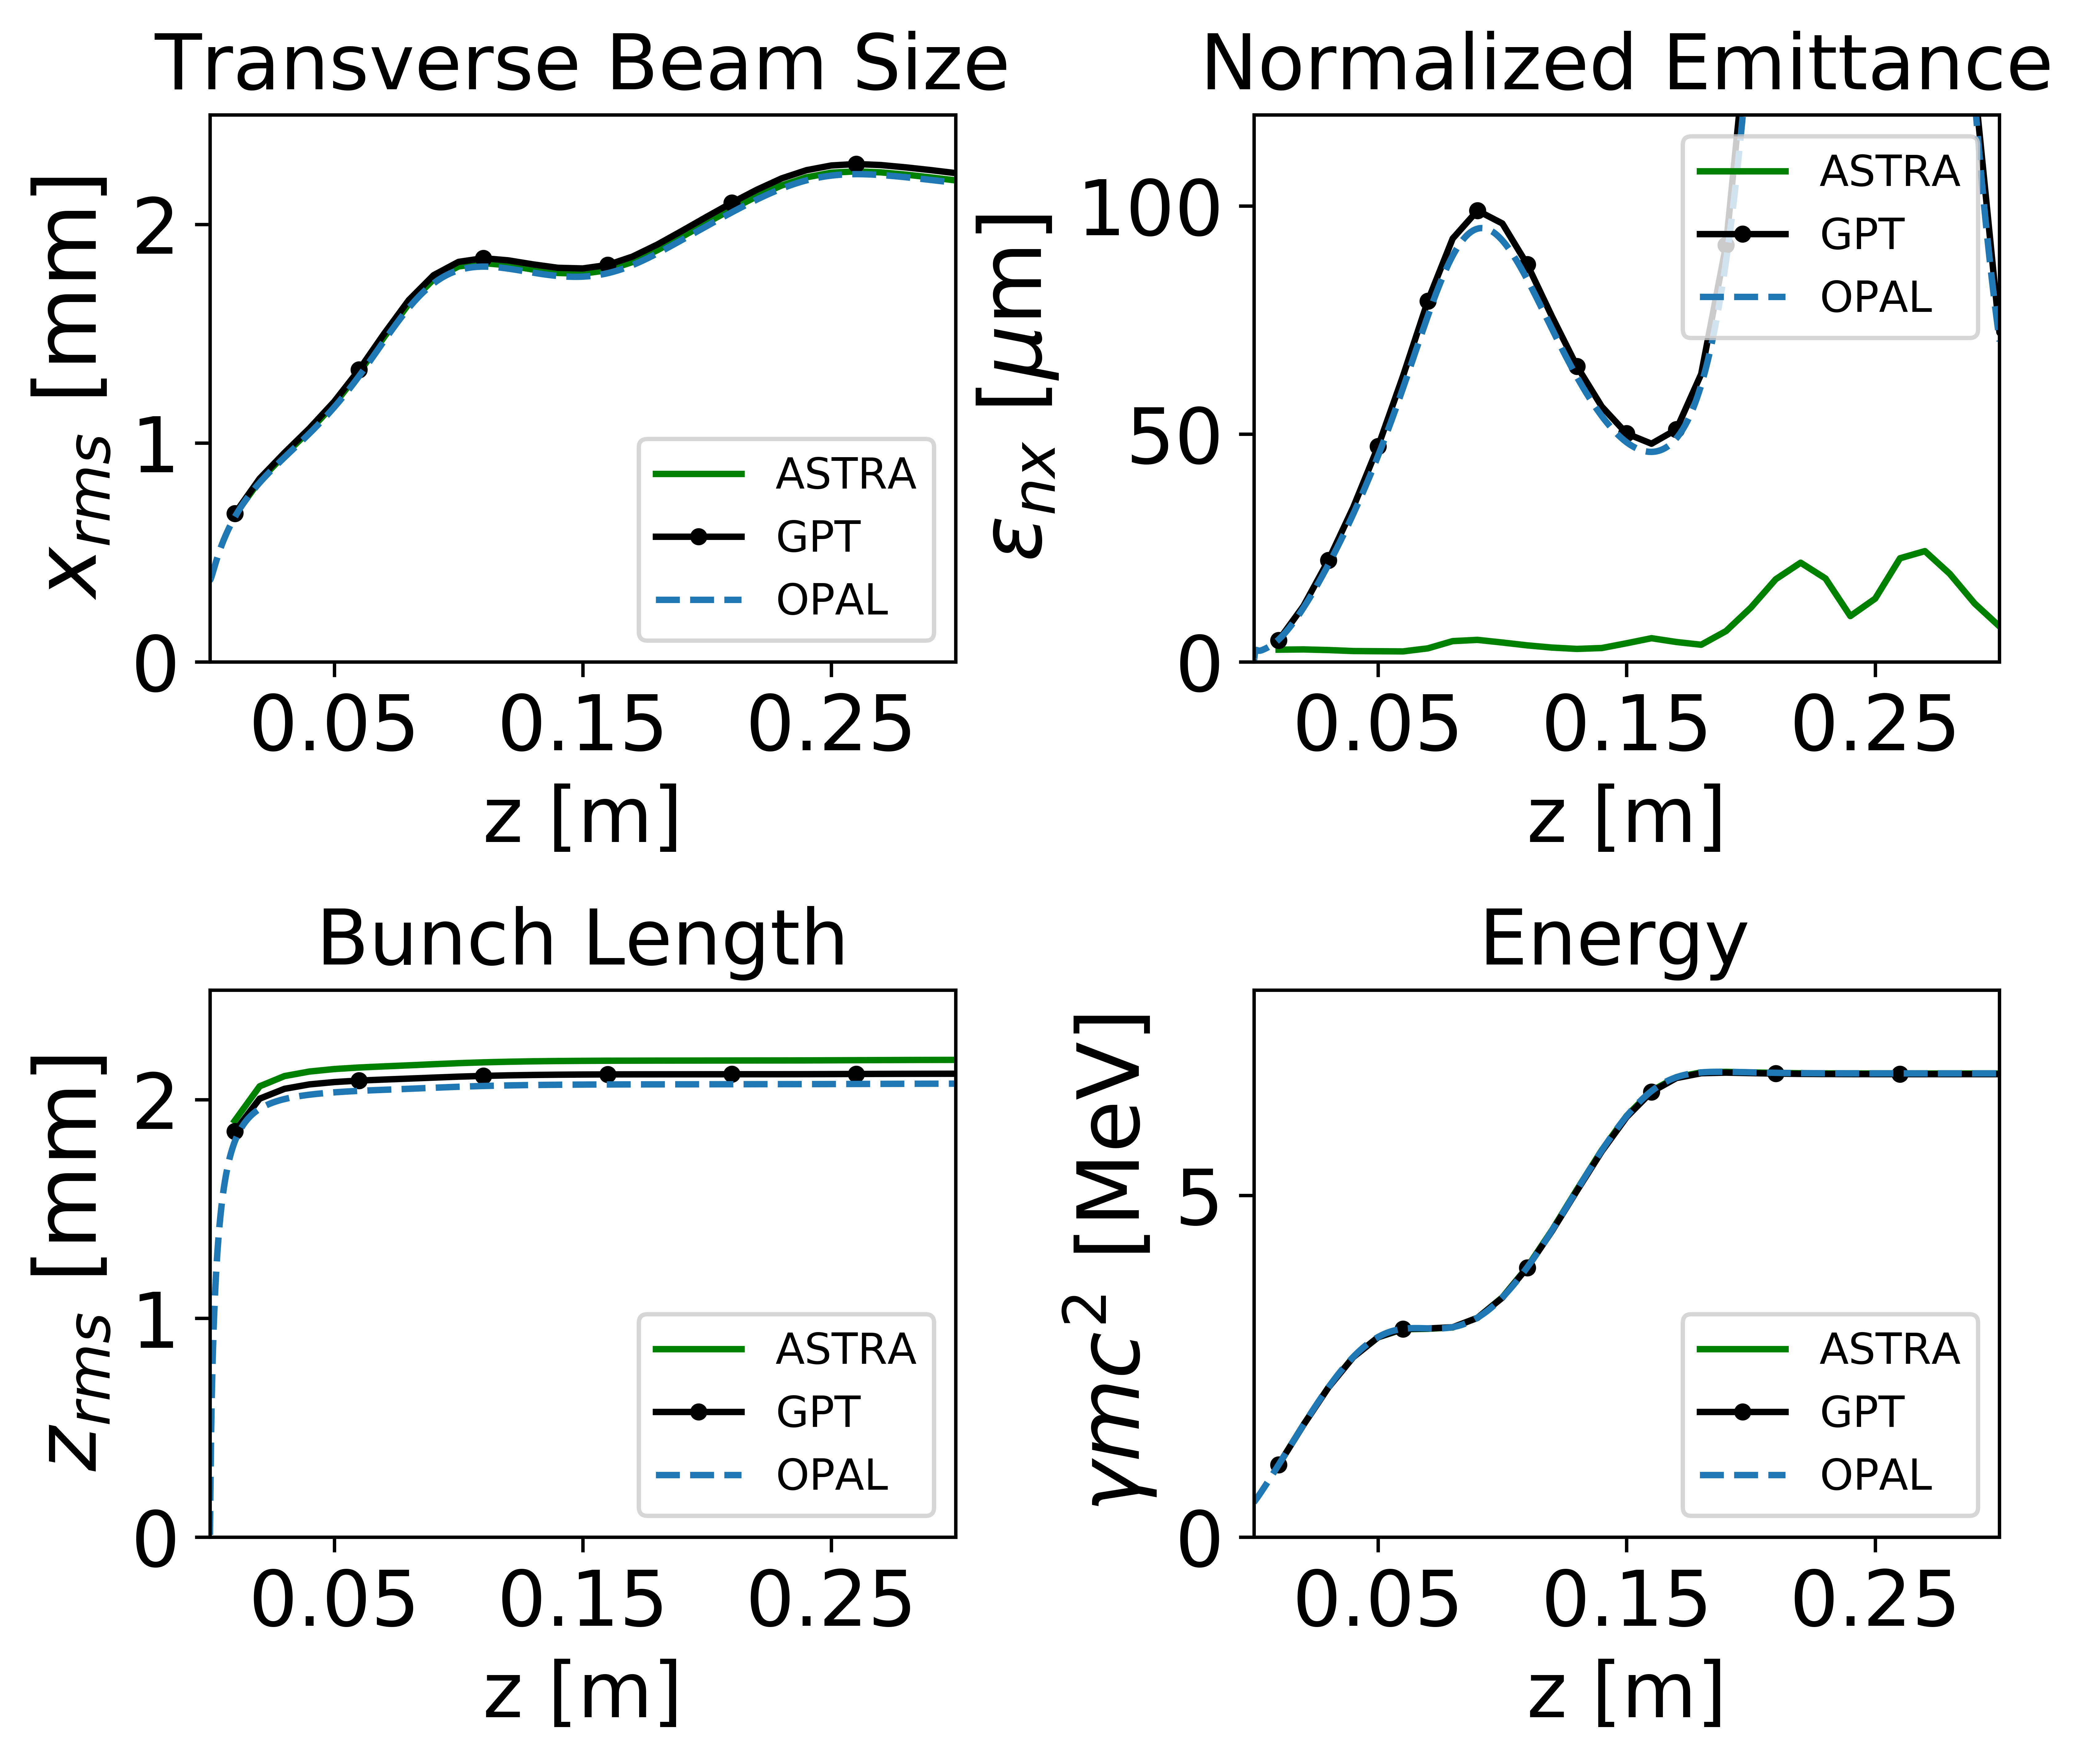
\includegraphics[width=0.8\textwidth]{images/benchmark_gun}
		\caption{Beam envelopes in the gun for benchmark between OPAL, ASTRA, and GPT.}
	    \label{fig:benchplot_gun}

        \vspace*{\floatsep}
        
		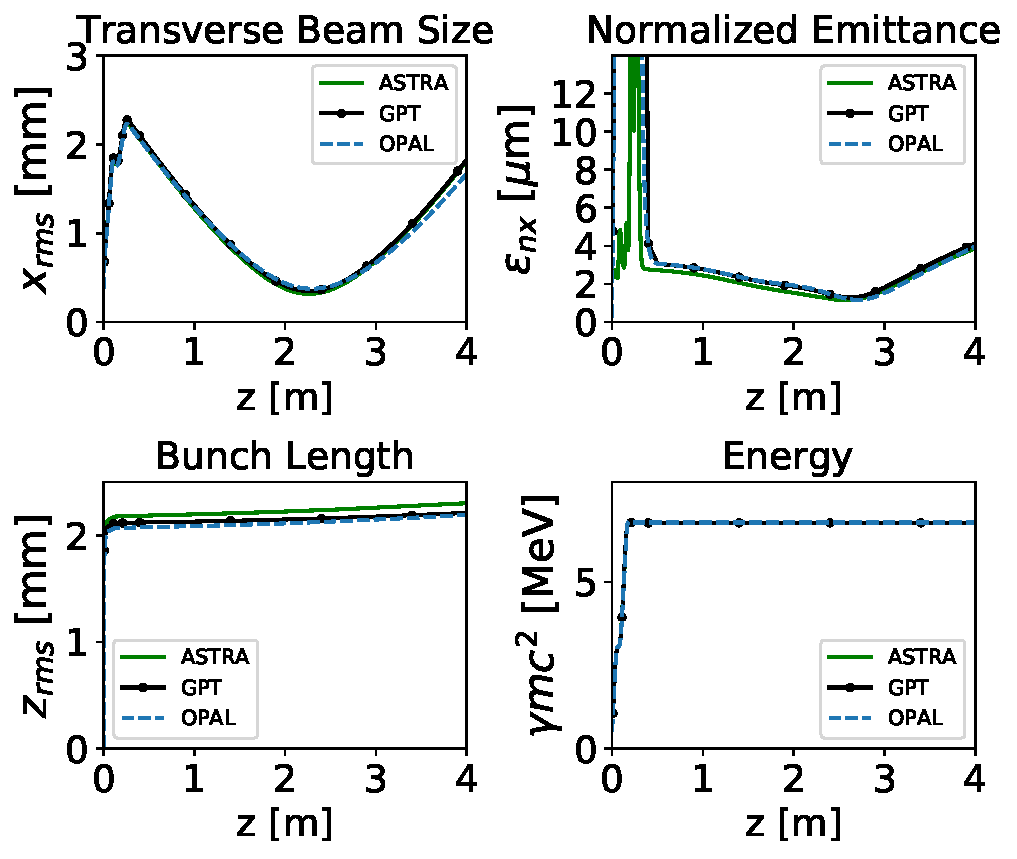
\includegraphics[width=0.8\textwidth]{images/benchmark_5m}
		\caption{Beam envelopes in drift for benchmark between OPAL, ASTRA, and GPT.}
	    \label{fig:benchplot_5m}
	\end{center}
\end{figure}

In general, the simulation results are in reasonable agreement 
and within expectations based on previous benchmarks \cite{codecompare}. 
See Figure~\ref{fig:benchplot_gun} and~\ref{fig:benchplot_5m} 
for a comparison of the beam envelopes generated by the three simulations in the gun and drift. 
The apparent disagreement of emittance between ASTRA and the other
two codes in the gun is because the former removes the angular momentum   
induced by the solenoid, while the other two codes do not. 
After the beam exits the solenoid, the emittance results  
are in good agreement, as shown in Figure~\ref{fig:benchplot_5m}.

\Subsection{Dipole Simulations}
Simulations of a hard edge dipole were done in GPT  
and OPAL-t in order to probe the CSR results.
Short mono-energetic bunches with a Gaussian energy distribution with zero initial transverse emittance  
were sent through the dipole. \lsnote{{\it If Gaussian in transverse parameter cannot be `zero emmittance'}} 
\nrnote{the Gaussian profile is in the longitudinal direction, I will double check}
Beam and dipole parameters are shown in Table~\ref{tab:benchcsr}. 
The CSR routine used in OPAL-t is based on the routine used in ELEGANT \cite{elegant}, 
which is known to assume the beam is ultra-relativistic. The CSR routine in GPT  
does not use the ultra-relativistic approximation ($\beta=1$) 
and as a result, works at all energies \cite{gptcsr}.  
Therefore, we expected the routines to match well at high energy and  
diverge at lower energy. Results of the CSR simulations are shown in Figure~\ref{fig:csr}  
As expected, the results between GPT and OPAL-t disagree at low energies. 
\begin{table}
	\begin{center}
		\caption{Input simulation parameters for CSR benchmark.}
		\label{tab:benchcsr}
		\begin{tabular}{l l} 
			\toprule
			\toprule
			\textbf{Parameter} & \textbf{Value} \\ 
			\midrule
			Dipole Length & \SI{0.3}{m} \\
			$\sigma_x =\sigma_y$ & \SI{1}{mm} \\
			$\sigma_z$ 			 & \SI{0.3}{mm} \\
			Bend Angle 			 & \SI{20}{^\circ} \\
			Energy (Mono-energetic)	 & \SI{2}{MeV} to \SI{100}{MeV} \\
			\bottomrule			
		\end{tabular}
	\end{center}
\end{table}
\begin{figure}
	\centering
	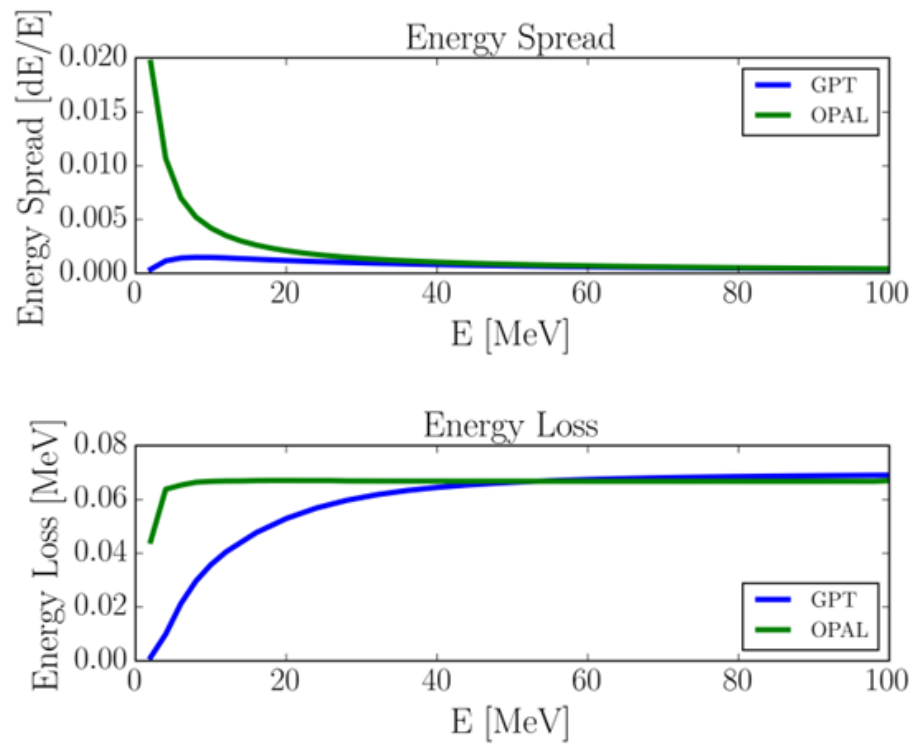
\includegraphics[width=0.5\textwidth]{./images/CSR}
	\caption{Results of CSR benchmark between OPAL and GPT.
	The codes agree well at high energies and diverge, as expected, at low energies.}
	\label{fig:csr}
\end{figure}

\Subsection{Benchmark Conclusion}
In summary, all three codes (OPAL, ASTRA, GPT), agreed well when modeling a photoinjector
with space charge effects, solenoid and RF fields.
OPAL and GPT also agree on energy loss and energy spread calculations at high energy.
At low energy they diverge, and GPT is more accurate because it calculates 
$\beta$ at all time vs. assuming the beam is relativistic.
Preference on which code to use depends more on ease of use 
and availability, \lsnote{especially for the AWA facility where $\beta\approx 1$.} 

\Section{Convergence Studies}

\lsnote{The OPAL code was chosen for modeling of the AWA after benchmarking was complete.}
Convergence runs were done for three parameters: 
time step, SC mesh size, and number of particles.  
Each case was tested in the gun using the same field maps and 
baseline settings that were used to compare SC in OPAL-t,  
ASTRA, and GPT in Section~\ref{sec:bench}. 
All OPAL-t simulations were run on 
sixteen cores, taking advantage of parallel calculations. 
The number of particles was varied from 20k to 3.2 million.  
The longitudinal parameters (energy,  bunch length)  
showed no variation, but there were slight deviations 
in the transverse emittance and beam size. The same results 
were observed when the time step was varied from 0.1 ps  to  10  ps.  
\lsnote{When the \sout{The}} grid size was changed from 32, 44, 46, and 64 cubed; 
again the results lacked any major discrepancies.  
In all cases, no appreciable differences were observed in the energy,
emittance, beam size, or bunch length. In  most  cases,  
if unreasonable  parameters  were chosen, 
OPAL-t would not complete the run (crash or hang up).  

From these runs, it was concluded that an appropriate starting point 
for mid fidelity simulations is 32 cubed grid with a time step
of 0.1 ps. The number of particles for such a run should be on the
order of 10's of thousands. On eight or sixteen compute cores
these simulations take on the order of minutes.

 
%%%%%%%%%%%%%%%%%%%%%%%%%%%%%%%%%%%%%%%%%%%%%%%%%%%%%%%%%%%%%%%%%%%%%%%%%%%%%%%%
%%%%%%%%%%%%%%%%%%%%%%%%%%%%%%%%%%%%%%%%%%%%%%%%%%%%%%%%%%%%%%%%%%%%%%%%%%%%%%%%
\Section{Optimization} \label{sec:opt}

Throughout the design process, optimization algorithms 
were used to study the beam parameters at the entrance of the TBA experimental area.
Minimizing the emittance and bunch length after the six cavity linac,
and choosing the optimal optics configuration for maximum beam transport 
were the main objectives of all optimization work.
The techniques used include model based, genetic,
and structure exploiting algorithms. 
 
Model-based, derivative-free, trust-region algorithms 
are increasingly popular for optimizing computationally 
expensive numerical simulations. \lsnote{The term model-based means that \sout{Where model-based refers
to the}} the simulation output \lsnote{is \sout{being}} used to construct a 
model. This can be a quadratic function as described later, 
or something more complex.
Derivative-free optimization indicates there is no one 
governing equation that defines all simulation output
for a given set of inputs. For example, there is no 
function for beam size \lsnote{that allows calucation of a derivative. \sout{that we can take the derivative of.}}
\lsnote{\sout{Calculating derivatives are in many} Many common optimization techniques calculate derivatives,} 
but \lsnote{this is} not applicable in situations of complex dynamics.
Finally, trust-region refers to the bounds on our input variables.
There are physical constraints on the magnet and RF values we 
can achieve in the real world. This information is used 
to bound the optimization work in a "trust-region", so that
effort is not wasted in an infeasible search space.
A strength of model based methods is their efficient use of function evaluations. 

After a model based method was implemented, a common technique was 
used as confirmation \lsnote{{\it Confirmation of what?}} and for exploratory work. \lsnote{{\it What type of exploratory work?}} The algorithm used for confirmation 
is called a genetic algorithm (GA). An implementation of this algorithm is
build into OPAL. GA's follow \lsnote{nature's \sout{natures}} lead as the name suggests.
A random sample is done, and the best points \lsnote{finish that thought ->} (give some criteria) \lsnote{ -> or delete.}
are selected. Those \lsnote{points \sout{point}} are then mixed to form a new "generation"
and a new round of simulations is started. This method continues
until some convergence criteria is met. While this method does 
produce results, and is widely used, it requires large amounts 
of computational resources to to reach convergence.
This is the most commonly used optimization in accelerator physics
at the moment. Preliminary designs 
for the TBA optics configuration were probed using the GA in to OPAL. 



\Subsection{Model Based Methods}
%\section{Optimization Algorithm}
% ----------------------------------------------------
The model-based algorithm was the first type of algorithm used to optimized the beam dynamics 
in two cases of interest at the AWA.
The first case was for lower beam charge, and used only the gun parameters for the optimization.  
The second case was for higher beam charge, and included parameters of the downstream linac as well as the gun.
In the first case,  the emittance of a \SI{1}{nC} electron 
bunch produced by the AWA rf photocathode gun 
was minimized by adjusting three parameters: rf gun phase, 
solenoid strength, and laser radius. The algorithm 
converged to a set of parameters that yielded an
emittance of \SI{1.08}{\um}. In the second case, 
the number of optimization parameters was expanded to model the complete AWA rf 
photoinjector (the gun and six accelerating cavities) at \SI{40}{nC}. 
The optimization algorithm was used in a Pareto study; which is a type of study that compares the 
trade-off between competing parameters, such as emittance and bunch 
length at the exit of the AWA \SI{70}{MeV} photoinjector. 

Model-based, derivative-free algorithms are frequently used to optimize
computationally expensive simulations due to their judicious use of function
evaluations. In cases specific to accelerator physics, 
beam properties at different operational parameters are observed;
these methods then build models of the unknown
function and minimize these models to identify candidate parameters to 
evaluate. Bounded Optimization BY Quadratic Approximation (BOBYQA)~\cite{bobyqa},
 is one such method that is available via the
NLopt~\cite{nlopt} package and was used in this study. 
Given a candidate set of optimal parameters $v^k$, BOBYQA
constructs a quadratic model using function values of points near $v^k$. 
This model is minimized in a neighborhood of $v^k$ in order to produce a point $\hat{v}$. 
If $\hat{v}$ has a smaller objective function value than $v^k$, 
the estimate of the optimum is updated to $\hat{v}$, and a new model is constructed. 
If $\hat{v}$ is not a sufficient improvement over $v^k$, 
the model around $v^k$ is improved. For more
information about derivative-free optimization, see~\cite{Conn2009a}.

The parameters $v^k$ are generated and supplied to OPAL-t~\cite{opal}. 
The optimization package NLopt and OPAL-t were used
in combination with Python code written at ANL with the help 
of Jeff Larson, to perform simulation evaluations and optimization.
All the files needed to replicate the results in this section are available at: 
$<$www.mcs.anl.gov/$\sim$jlarson/AWA$>$.  

\Subsection{Optimization Parameters}
% ----------------------------------------------------
When optimizing the gun, three parameters $v^k$ were varied: 
solenoid strength ($S_3$), gun phase ($\phi_g$), 
and laser radius ($R$) of a uniform photon distribution. 
The minimized objective was emittance ($\epsilon_x$).
(The reference phase of the gun is defined as $0^{\circ}$ at maximum accelerating voltage.) 
When optimizing the gun and the entire linac, seven additional parameters were 
varied: the longitudinal duration of the laser pulse, defined at full width at half maximum ($T$)
and accelerating cavity phases ($\phi_L$). The optimization parameters and
bounds are given in Table~\ref{tab:parameters}; we denote the set of
ten optimization parameters as $v=[S_3, \phi_g, R, T, \phi_L]$, where 
$\phi_L=[\phi_{L_1},\ldots,\phi_{L_6}]$ represents the phase of each linac cavity $L_1$-$L_6$. 
\nrnote{need to fix footnotes and superscripts for table 3.3}
\begin{table}
	\caption{\label{tab:parameters} Parameter bounds for gun and linac optimization.}
	\begin{center}
		\begin{tabular}{ l *{3}{c}} 
			\toprule
			\textbf{Variable} & \textbf{Range} & \textbf{Unit} \\
			\midrule
			Solenoid Strength & $ 0 \le S_3 \le 440$  & amps \\
			Phase of Gun & $-60 \le \phi_g \le 60$  & degrees \\
			Laser Radius  & $0.1 \le R \le 30$  & mm \\
			Laser FWHM & $2 \le T \le $10  & ps \\
			Cavity Phase  & $-20 \le \phi_L \le 20$  & degrees \\
			\bottomrule	
		\end{tabular}
	\end{center}
\end{table}


\Subsection{Gun Simulations Using BOBYQA} \label{sec:gunbobyqa}
%\section{Gun Optimization}
% ----------------------------------------------------
There has been work done by other groups to optimize 1.5 cell rf guns
at \SI{1}{nC}~\cite{pitz}. The known solution from that work was used as 
a baseline test of BOBYQA when applied to this accelerator application.
An optimization of the single objective emittance ($\epsilon_x$) was 
performed over a length of \SI{5}{m}. 
All linacs were turned off and only gun parameters were varied. 
Non-varying parameters are listed in table~\ref{tab:gun}; 
their values are based on realistic parameters at PITZ and AWA~\cite{pitz, benchmark}.

Local optimization runs were started using five points 
\lsnote{OK, then do you mean `each with a different selection of values for the optimization parameters'?  {\it If yes, add that here.}} 
\nrnote{No, it was a total of five points with various simulation inputs.}with various 
differences from the optimum value. The optimization runs converged 
(in less than 100 function evaluations) to a parameter set ($S_3=\SI{269}{A}$,
$\phi_g=\SI{-3.0}{^{\circ}}$, and $R=\SI{0.6}{mm}$) with an emittance of $\SI{1.08}{\um}$.
An exhaustive search of the parameter space was not done, and there may be other local minima that were not found.
However, the results match expectations based on the literature. 
\begin{table}%[h] 
	\caption{\label{tab:gun} Non-varying parameters for gun optimization.}
	\begin{center}
		\begin{tabular}{lll}
			\toprule
			\textbf{Parameter} & \textbf{Value} \\
			\midrule
			Charge  & \SI{1}{nC} \\
			Gradient & \SI{60}{MV/m} \\
			Laser FWHM & \SI{20}{ps} \\
			Laser Rise and Fall Time & \SI{6}{ps} \\
			Kinetic Energy at Cathode  & \SI{0.55}{eV} \\
			$S_1$ and $S_2$ & \SI{550}{A} \\
			\bottomrule
		\end{tabular}
	\end{center}
\end{table}

\Subsection{Linac Optimization}\label{sec:linacopt}
Next we performed a multiobjective optimization of the linac (Figure~\ref{fig:beamline}), 
by adjusting the ten parameters in table~\ref{tab:parameters}. The charge was set to \SI{40}{nC}
and was chosen to match upcoming two-beam acceleration experiments~\cite{tba2017}. 
Two objectives were considered: emittance and bunch length ($\sigma_z$). 
The location of interest is $z_1=\SI{12.51}{m}$, as this is the entrance of the first 
quadrupole magnet after the linac. \lsnote{Optimization was required only for the horizontal emittance, $\epsilon_{x}$.  This is because there were no asymmetric focusing elements in the linac, and the beam is round, $\epsilon_{x}=\epsilon_{y}$. 
\sout{We optimize $\epsilon_{x}$ instead of $\epsilon_{xy}$ because no asymmetric focusing elements were used in the linac.}}  The non-varying parameters for all linac simulation runs are shown in table~\ref{tab:linac}.  \lsnote{The particle distribution initally emitted from the cathode is generated within OPAL using input parameters such as the cathode material, the work function and the laser energy.  In this case, \sout{
The model used simulated emission
from} a Cs$_2$Te cathode} \lsnote{was used with \sout{using}} a laser \lsnote{of \sout{with}} initial kinetic energy of \SI{4}{eV}. 
These are typical operating conditions at AWA. 


\def \gunleft {-1.0}
\def \gunright {0.3}
\def \loneright {1.0}
\def \ltworight {3.5}
\def \lthreeright {5.0}
\def \lfourright {7.0}
\def \lfiveright {8.5}
\def \lsixright {10}
\begin{figure*}
	\begin{center}
		
		\begin{tikzpicture}[scale=0.95]
		%Gun drawings
		\draw[fill=orange, very thick, rounded corners =0.1cm] (\gunleft,0.5)rectangle (\gunright,1.5) node[pos=.5, white] {\textbf{Gun}} ;
		
		%S1
		\node[] at (-1.3,2.9) {$S_1$};
		\draw[ultra thick, fill=black!60!green] (-1.4,-0.5)rectangle  (-1.0,0.5) node[pos=.5, white] {} ;
		\draw[black, ultra thick] (-1.4,-0.5) -- (-1.0,0.5);
		\draw[black, ultra thick] (-1.4,0.5) -- (-1.0,-0.5);
		\draw[ultra thick, fill=black!60!green] (-1.4,1.5)rectangle  (-1.0,2.5) node[pos=.5, white] {} ;
		\draw[black, ultra thick] (-1.4,1.5) -- (-1.0,2.5);
		\draw[black, ultra thick] (-1.4,2.5) -- (-1.0,1.5);
		%S2
		\node[] at (-0.8,2.9) {$S_2$};
		\draw[ultra thick, fill=black!60!green] (-1.0,-0.5)rectangle  (-0.6,0.5) node[pos=.5, white] {} ;
		\draw[black, ultra thick] (-1.0,-0.5) -- (-0.6,0.5);
		\draw[black, ultra thick] (-1.0,0.5) -- (-0.6,-0.5);
		\draw[ultra thick, fill=black!60!green] (-1.0,1.5)rectangle  (-0.6,2.5) node[pos=.5, white] {} ;
		\draw[black, ultra thick] (-1.0,1.5) -- (-0.6,2.5);
		\draw[black, ultra thick] (-1.0,2.5) -- (-0.6,1.5);
		
		%S3
		\node[] at (0.2,2.9) {$S_3$};
		\draw[ultra thick, fill=black!60!green] (-0.1,-0.5) rectangle  (0.3,0.5) node[pos=.5, white] {};
		\draw[black, ultra thick] (-0.1,-0.5) -- (0.3,0.5);
		\draw[black, ultra thick] (-0.1,0.5) -- (0.3,-0.5);
		\draw[ultra thick, fill=black!60!green] (-0.1,1.5) rectangle  (0.3,2.5) node[pos=.5, white] {};
		\draw[black, ultra thick] (-0.1,1.5) -- (0.3,2.5);
		\draw[black, ultra thick] (-0.1,2.5) -- (0.3,1.5);
		%Linac drawings 
		\draw[fill=blue, ultra thick, rounded corners =0.1cm] (\loneright,0)rectangle  ({\loneright+0.84},2) node[pos=.5, white] {$L_1$} ;
		\draw[fill=blue, ultra thick, rounded corners =0.1cm] (\ltworight,0)rectangle  ({\ltworight+0.84},2) node[pos=.5, white] {$L_2$};
		\draw[fill=blue, ultra thick, rounded corners =0.1cm] (\lthreeright,0)rectangle ({\lthreeright+0.84},2) node[pos=.5, white] {$L_3$};
		\draw[fill=blue, ultra thick, rounded corners =0.1cm] (\lfourright,0)rectangle ({\lfourright+0.84},2) node[pos=.5, white] {$L_4$};
		\draw[fill=blue, ultra thick, rounded corners =0.1cm] (\lfiveright,0)rectangle ({\lfiveright+0.84},2) node[pos=.5, white] {$L_5$};
		\draw[fill=blue, ultra thick, rounded corners =0.1cm] (\lsixright,0)rectangle ({\lsixright+0.84},2) node[pos=.5, white] {$L_6$};
		\draw[very thick] (\gunleft,-1.5) -- (14,-1.5);
		\draw[latex-latex] (\gunleft,-1.5) -- (14,-1.5) ; 
		\foreach \x in  {0.3, 1.0, 3.5, 5.0, 7.0, 8.5, 10, 12.5} %tick marks
		\draw[shift={(\x,-1.5)},color=black] (0pt,3pt) -- (0pt,-3pt);
		\foreach \x in {0.3, 1.0, 3.5, 5.0, 7.0, 8.5, 10, 12.5}
		\draw[shift={(\x,-1.7)},color=black] (0pt,0pt) node[below] 
		{$\x$};
		
		\node[draw, fill=yellow, star, star points=5, star point ratio=0.6, minimum size=0.6cm]
		at (12.5,1.0) {$z_1$};
		\end{tikzpicture}
	\end{center}
	\caption{Layout of the AWA linac. The \SI{70}{MeV} AWA rf photoinjector 
		is an rf gun followed by a linac with six rf accelerating cavities, 
		labeled $L_1$-$L_6$ \cite{Power:2010zza}.  The cavity phases are controlled independently. 
		The 1.5 cell rf gun operates at \SI{1.3}{GHz} with three solenoids 
		and a Cs$_{2}$Te photocathode excited by a \SI{248}{nm} UV laser.  
		Solenoid 1 ($S_1$) is used to buck the field at the cathode,
		while the other two solenoids ($S_2$ and $S_3$) are used for emittance compensation.  
		Tick marks are located at the exit of the gun, entrance of
		each accelerating cavity, and location of optimization.}
	\label{fig:beamline} 
\end{figure*} 
\begin{table}%[h] %or [hbt] ?
	\caption{\label{tab:linac} Non-varying parameters for linac optimization.}
	\begin{center}
		\begin{tabular}{lll}
			\toprule
			\toprule
			\textbf{Parameter} & \textbf{Value} \\
			\midrule
			Charge  & \SI{40}{nC} \\
			Laser Rise and Fall Time & \SI{1.0}{ps} \\
			Gun Gradient & \SI{70}{MV/m} \\
			$S_1$ and $S_2$ & \SI{550}{A}\\
			Cavity Gradient $L_1$--$L_4$ & \SI{25}{MV/m} \\
			Cavity Gradient $L_5$--$L_6$ & \SI{27}{MV/m} \\
			\bottomrule
		\end{tabular}
	\end{center}
\end{table}

A 1,000 point sample of linac parameters were drawn from the domain
in table~\ref{tab:parameters} and simulated. Of these, 132 simulations completed
without error, and the emittance and bunch length at $z_1=\SI{12.51}{m}$ was
recorded for each of these points. From the sample of the 132 successful simulations 
the minimum and maximum values of emittance and bunch length
were found (i.e: $\epsilon_{\min}$ and $\epsilon_{\max}$). 
The raw $\epsilon_x(v,z_1)$ and $\sigma_z(v,z_1)$ sample values were then
shifted and scaled to produce $\bar{\epsilon}_x(v,z_1)$, and $\bar{\sigma}_z(v,z_1)$,
which have a minimum value of 0 and a maximum value of 1 over the 132-point sample set. That is, 
\begin{equation}
\bar{\epsilon}_x (v,z_1) = \frac{ \epsilon_x (v,z_1) - \epsilon_{\min} } { \epsilon_{\max} - \epsilon_{\min} }
\label{eq:scale}
\end{equation} 
and $\bar{\sigma}_z (v,z_1)$ is defined similarly.
This scaling is done in order to remove the difference in the units between
emittance and bunch length when optimizing.

With the scaled values of $\bar{\epsilon}_x$ and $\bar{\sigma}_z$, a sequence
of eleven optimization problems were solved by minimizing,
\begin{equation}
f(v,w) = w \,\bar{\epsilon}_x(v,z_1) + (1-w)\, \bar{\sigma}_z(v,z_1)
\label{eq:newobj}
\end{equation}
for $w \in \left\{ 0, 0.1, \ldots, 1 \right\}$. 
For each weight $w$, BOBYQA was started from the sample point with the 
smallest value of $f(v,w)$.  From the initial random sample, six unique starting points were chosen. 
(There were fewer starting points than weights because some samples had the smallest objective value for multiple weights. 
For example, the smallest values of $f(v,0.4)$, $f(v,0.5)$, and $f(v,0.6)$ occurred when at the eighteenth sample point.)
Some $f(v,w)$ values also had one or more linac phases near the initial $\pm20^{\circ}$ boundary. 
The $\phi_L$ boundary was expanded to $\pm40^{\circ}$ for those BOBYQA runs.

\Subsection{Pareto Front for AWA Linac}
%\section{Pareto Front for AWA Linac} 
% ----------------------------------------------------
Since multiple objectives are under consideration in this case, a
trade-off analysis is necessary. 
\begin{figure}%[h]
	\begin{center}
		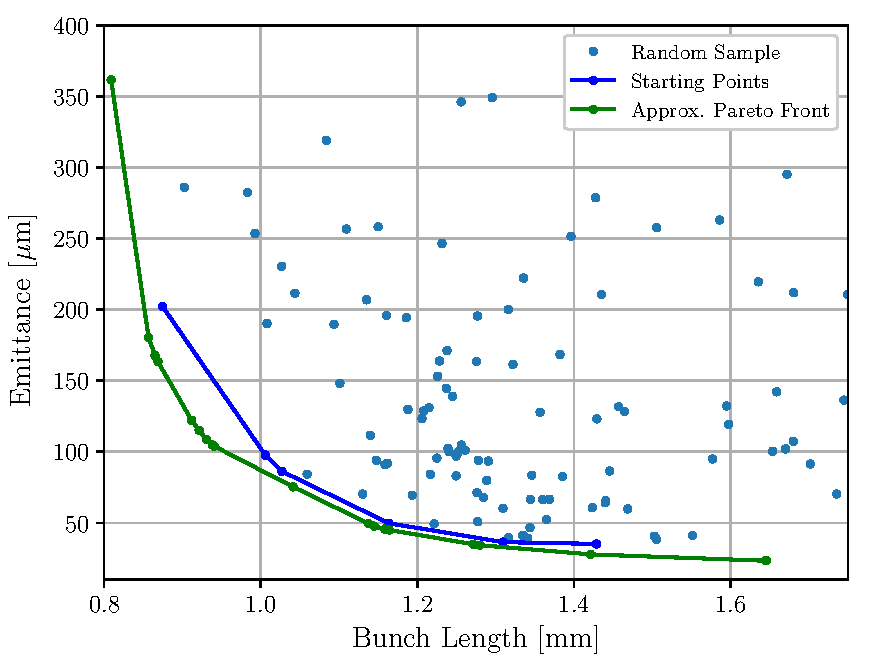
\includegraphics[width=0.75\textwidth]{images/THPAB155f1}
		\caption{Random sample results, starting sample points, and resulting approximate Pareto front for the linac at \SI{40}{nC}. The Pareto front is the result of all BOBYQA evaluations.}
		\label{fig:pareto}
	\end{center}
\end{figure}
This can be aided by examining a Pareto front: the set of parameters 
for which no other point exists that is better with respect to both objectives~\cite{ehrgott2006multicriteria}.
In Figure~\ref{fig:pareto}, blue dots show the emittance and bunch length for the
evaluated random sample. The sample points for which no other point has better
emittance and bunch length are connected with a blue line. BOBYQA was started
from these points, as described above, producing the green approximate Pareto front. 

The number of simulation evaluations needed to obtain convergence
in the BOBYQA runs varied from a minimum of 107 evaluations to a maximum of 208 
evaluations. In order to generate the Pareto front in
Figure~\ref{fig:pareto}, a total of 2,492 simulation evaluations were completed.
Most simulation evaluations took approximately 7 minutes, using 16 cores and 100,000 particles. These numbers are driven by the amount of time OPAL-t needs to simulate the beam line. 

The best-found objective value through each BOBYQA run is shown in Figure~\ref{fig:iterations}. 
Weight 0.0 and 1.0 are negative due to the scaling in Equation~(\ref{eq:scale}). While the weights, $w$, are always nonnegative, 
$\bar{\epsilon}_x (v,z_1)$ or $\bar{\sigma}_z(v,z_1)$ will be negative if BOBYQA finds a point with a value of 
$\epsilon_x(v,z_1)$ or $\sigma_z(v,z_1)$ that is less than $\epsilon_{\min}$ or $\sigma_{\min}$ from the initial sample. 
\begin{figure}%[h]
	\begin{center}
		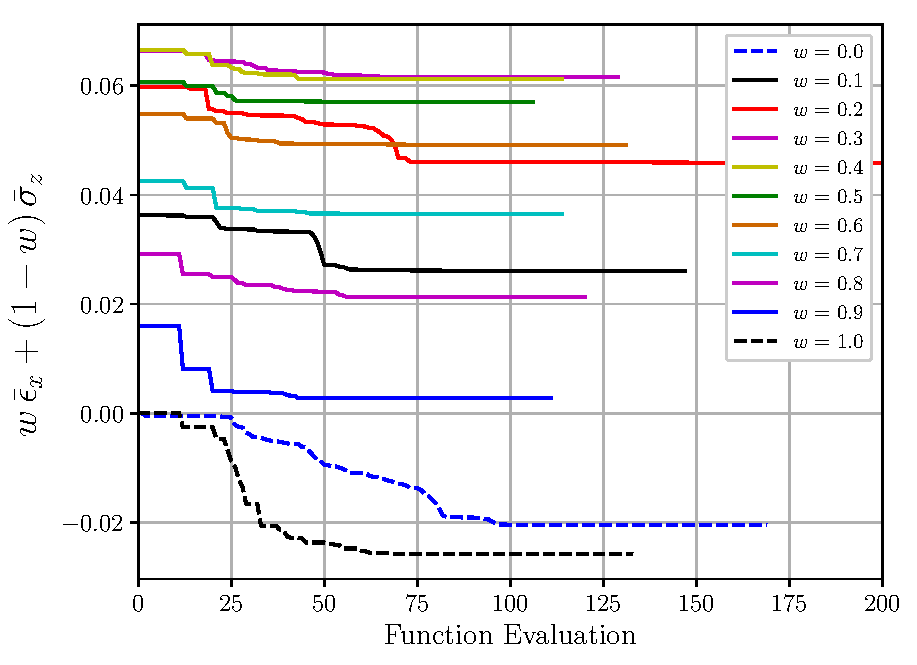
\includegraphics[width=0.75\textwidth]{images/THPAB155f2}
		\caption{\label{fig:iterations}Minimum observed objective function values during eleven BOBYQA runs at \SI{40}{nC}.}
	\end{center}
\end{figure}

We note that seven of the BOBYQA runs converged to emittance values
between \SI{20}{\mu m} and \SI{50}{\mu m}, which is shown in Figure~\ref{fig:trade} 
along with gun phase and bunch length for each of the 11
optimized points. We annotate Figure~\ref{fig:trade} with $T$ because that parameter 
shows strong correlation with the gun phase. Other optimized parameters such as the laser radius were found to stay within a 
narrow range (\SIrange{10}{16}{mm}).  
\begin{figure}%[h]
	\begin{center}
		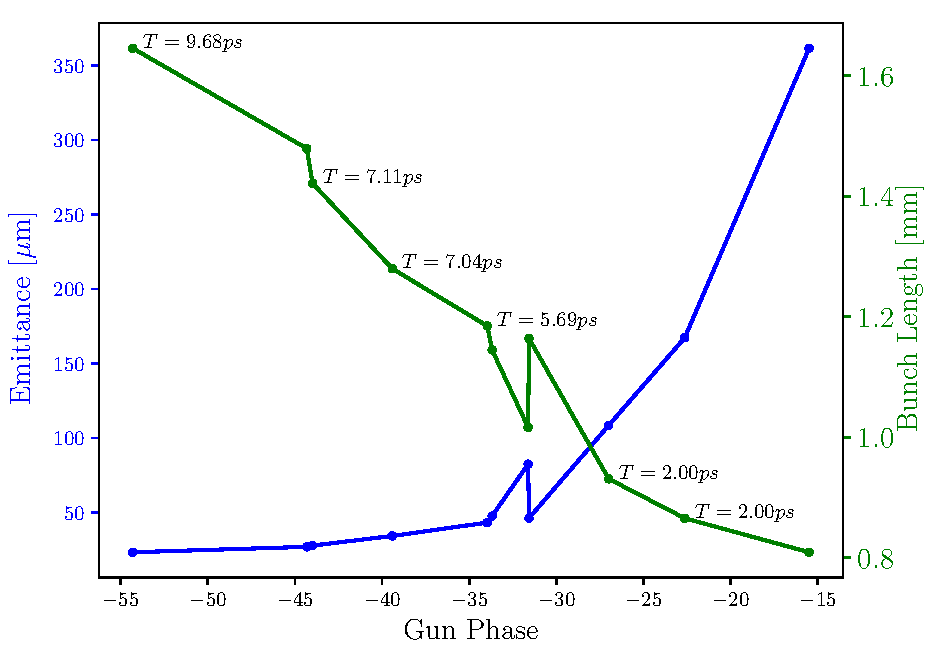
\includegraphics[width=0.75\textwidth]{images/THPAB155f3}
		\caption{\label{fig:trade}Bunch length and emittance vs.~gun phase at each optimized point in the Pareto front for the linac at \SI{40}{nC}. The phase of the max energy gain is 0$^{\circ}$.}
	\end{center}
\end{figure}


The optimized linac phases maximize energy gain while minimizing the energy spread.
The energy spread of the beam exiting the gun depends strongly on $\phi_g$.
There are three distinct regions where the optimized points had similar gun phases 
(less than $\pm10^{\circ}$) which resulted in nearly identical linac phases. For example:  
all six phases, $\phi_L$, varied by less than $10^{\circ}$ for $w \in \left\{ 0, 0.1\right\}$,
less than $5^{\circ}$ for $w \in \left\{ 0.4, 0.5, 0.6\right\}$, 
and less than $10^{\circ}$ for $w \in \left\{ 0.7, 0.8, 0.9\right\}$.
This indicates optimized linac phases may benefit a range of gun settings during operation. 


\Subsection{Lessons Learned from BOBYQA Work}
Using an AWA beam line as the simulation model, we used the BOBYQA algorithm 
to optimize the emittance produced by the gun at \SI{1}{nC}.
Using the same algorithm, we performed a multiobjective analysis for the linac at \SI{40}{nC}. 
A Pareto front comparing the trade-off between bunch length and emittance was generated for the linac. 
In total, only 2,492 simulation evaluations were needed to produce the approximate Pareto front.
From this work a few key take aways are clear. First, larger laser radius
is uniformly better for high charge. i.e large radius helps lower emittance.
The second clear results is alternating the phases in the linac can control 
the energy spread created by the gun, i.e. running off crest in the linac 
can reduce the energy spread significantly.

%%%%%%%%%%%%%%%%%%%%%%%%%%%%%%%%%%%%%%%%%%%%%%%%%%%%%%%%%%%%%%%%%%%%%%%%%%%%%%%%
%%%%%%%%%%%%%%%%%%%%%%%%%%%%%%%%%%%%%%%%%%%%%%%%%%%%%%%%%%%%%%%%%%%%%%%%%%%%%%%%
\Subsection{Genetic Algorithm: NSGA-II} \label{sec:ga}
%%%%%%%%%%%%%%%%%%%%%%%%%%%%%%%%%%%%%%%%%%%%%%%%%%%%%%%%%%%%%%%%%%%%%%%%%%%%%%%%
%%%%%%%%%%%%%%%%%%%%%%%%%%%%%%%%%%%%%%%%%%%%%%%%%%%%%%%%%%%%%%%%%%%%%%%%%%%%%%%%
While the model based results are promising, 
GA's are the most commonly used type of optimization algorithm in the accelerator community.
In particular the Non-dominated Sorting Genetic Algorithm II (NSGA-II)~\cite{NSGA}, 
is the implementation that is most commonly used.
\nrnote{add another sentence about NSGAII details.}
To validate that the model based method was giving comparable results to what a GA would give, 
a low fidelity version of the linac simulation in Section~\ref{sec:linacopt} was formulated.
This fidelity change included reducing the number of particles and grid points. 
The boundaries on the design variables were also reduced to ensure only 
feasible simulation points were evaluated.

Figure~\ref{fig:GAvsModel} clearly shows the optimized simulations results from 
the GA and model based method are similar. Both methods gave desirable 
results for the linac optimization problem. 
The main difference between the two methods is the amount of computational 
resources needed, see the comparison in Table~\ref{tab:optcompare}.
Note, that as a general \lsnote{rule of thumb, \sout{r.o.t.}} most people simulate at least 100 generations, before stopping a GA.
\lsnote{This suggests that while \sout{These results suggest}} the model based method and GA will arrive at 
the same conclusion, \lsnote{\sout{per say, but at different times.} there will likely be a time difference for completion. {\it Is this significant?}}
\begin{figure}
	\centering
	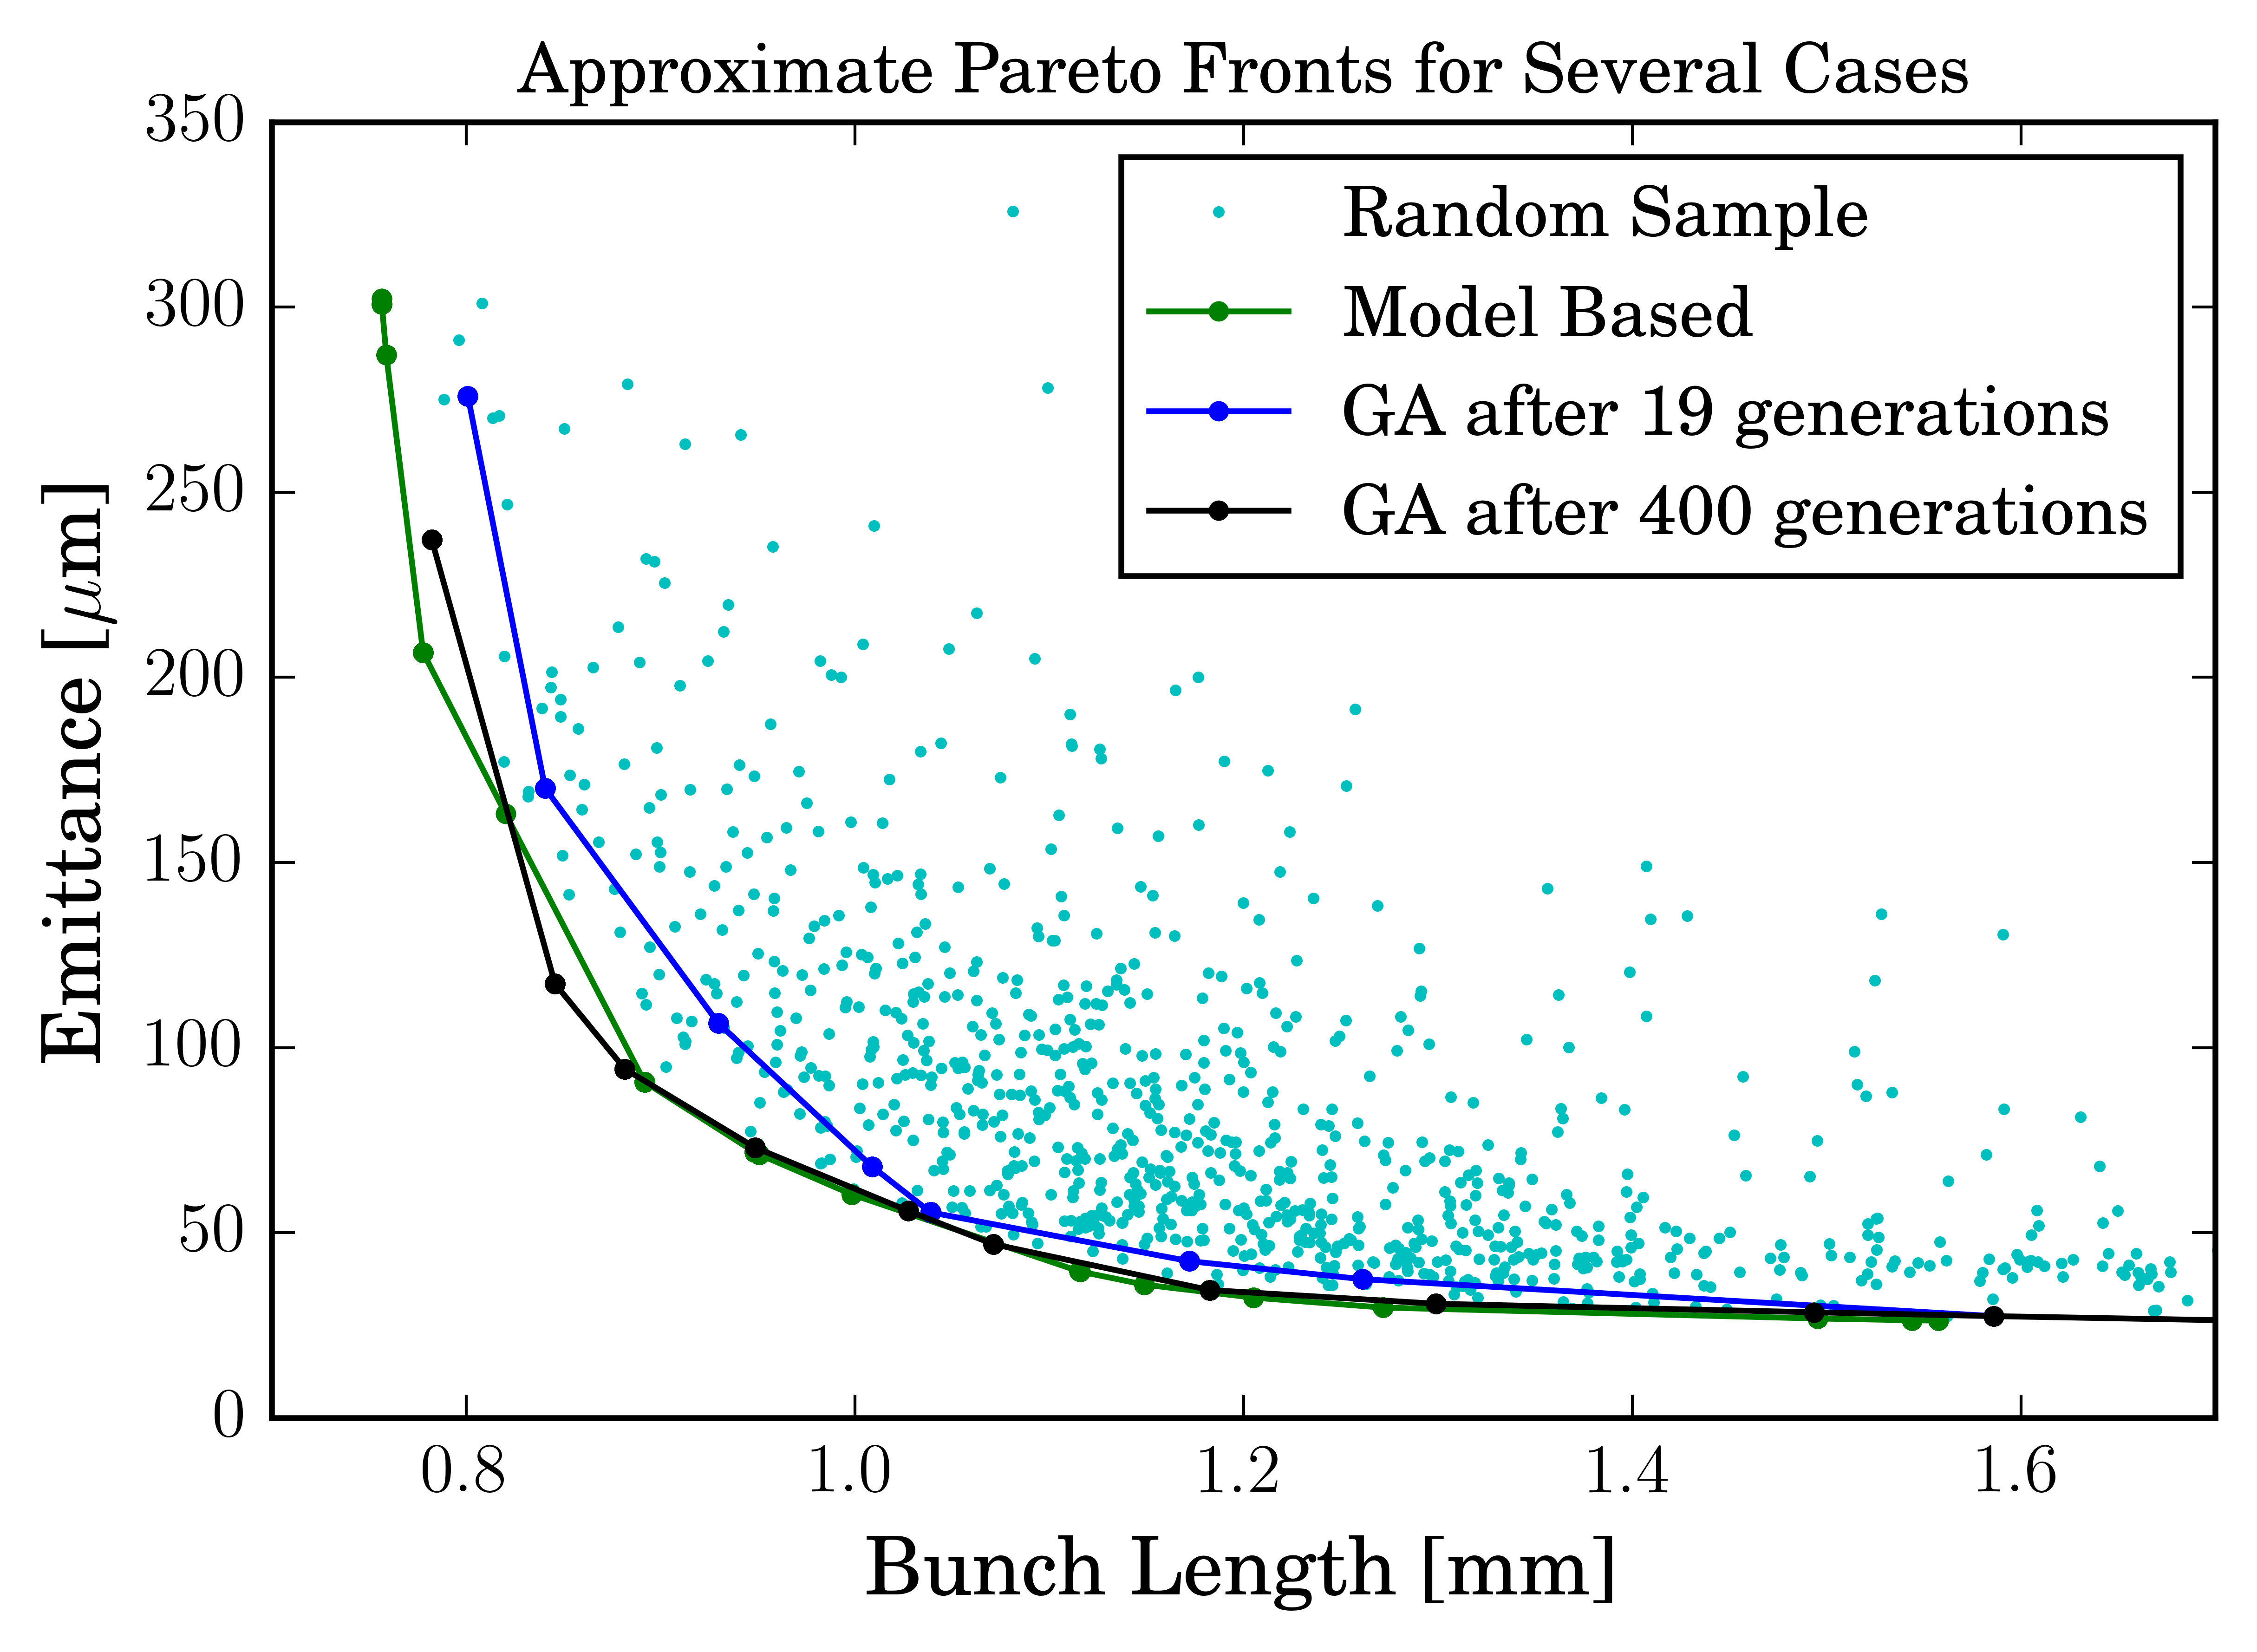
\includegraphics[width=0.75\textwidth]{./images/model_vs_ga}
	\caption{Comparison of model based and GA simulations results.}
	\label{fig:GAvsModel}
\end{figure}
\begin{table}[h] %or [hbt] ?
	\caption{Number of simulation evaluations for model based and GA optimizations.
	These numbers correspond to the lines in Figure~\ref{fig:GAvsModel}.}
	\label{tab:optcompare}
	\begin{center}
		\begin{tabular}{lcc}
			\toprule
			\toprule
			\textbf{Optimization} & \textbf{Number of Simulations} & \textbf{Compute Hours} \\
			\midrule
			Model Based  		& 2393  & 79.8 \\
			GA 19 Generations 	& 2432  & 81.1 \\
			GA 200 Generations 	& 25600 & 853.3\\
			GA 400 Generations 	& 51200 & 1706.7\\
			\bottomrule
		\end{tabular}
	\end{center}
\end{table}

\lsnote{{\it What you are trying to say below goes in the chapter summary.  You can use it as the final wrap up, something like `Validation of OPAL T and initial optimization studies provided a tool to design the TBA experimental area.  This work is described in the next chapter.}}
Next, work began on designing the TBA experimental area. 
Initial probes into this problem were done using the genetic algorithm
implemented in OPAL-t~\cite{optpilot}. Details of this work can be found in Chapter~\ref{chp:4}.

\Section{Chapter Summary}

PIC simulations of the AWA drive line are essential to the TBA project. \lsnote{{\it say why}}
A new code, OPAL-t, was \lsnote{investigated\sout{investigate}} as an alternative to ASTRA and GPT. 
The benefits of OPAL include \lsnote{being \sout{it is}} free and \lsnote{being able to run on a} parallel \lsnote{platform}.
A benchmark was done to ensure that OPAL \lsnote{gave results consistent with \sout{was being used correctly in comparison to}} other codes used by members of the AWA.
No major discrepancies were found in the space charge and CSR algorithms.
Although, \lsnote{note that} the OPAL CSR routine can not be used for low energy beams.
Convergence studies were also done to determine base line computational 
parameters for future simulations.
\lsnote{After benchmarking, \sout{Moving forward}} all PIC simulations of the TBA beam line \lsnote{in this work} were performed using OPAL-t on clusters provided by ANL.

Next, optimization \lsnote{to find \sout{work began to prepare}} a set of operating parameters for
\SI{40}{nC} TBA experiments \lsnote{was done. \sout{This work included using the} A} model based method BOBYQA \lsnote{was used} to optimize the gun and linac. \lsnote{{\it You need a few sentences about the resulting optimized beam parameters and whether they make sense.}}
Validation of the model based \lsnote{method \sout{methods}} was done \lsnote{by doing a comparison} with the commonly used GA method. The results agreed well, and \lsnote{suggest \sout{suggested} that } the model based 
methods require fewer computational resources than a GA. 






